% Autor: Leonhard Segger, Alexander Neuwirth
% Datum: 2017-10-30
\documentclass[
	% Papierformat
	a4paper,
	% Schriftgröße (beliebige Größen mit „fontsize=Xpt“)
	12pt,
	% Schreibt die Papiergröße korrekt ins Ausgabedokument
	pagesize,
	% Sprache für z.B. Babel
	ngerman
]{scrartcl}

% Achtung: Die Reihenfolge der Pakete kann (leider) wichtig sein!
% Insbesondere sollten (so wie hier) babel, fontenc und inputenc (in dieser
% Reihenfolge) als Erstes und hyperref und cleveref (Reihenfolge auch hier
% beachten) als Letztes geladen werden!

\usepackage{tikz}
\usetikzlibrary{calc,patterns,angles,quotes} % loads some tikz extensions\usepackage{tikz}
\usetikzlibrary{babel}

% Silbentrennung etc.; Sprache wird durch Option bei \documentclass festgelegt
\usepackage{babel}
% Verwendung der Zeichentabelle T1 (Sonderzeichen etc.)
\usepackage[T1]{fontenc}
% Legt die Zeichenkodierung der Eingabedatei fest, z.B. UTF-8
\usepackage[utf8]{inputenc}
% Schriftart
\usepackage{lmodern}
% Zusätzliche Sonderzeichen
\usepackage{textcomp}

% Mathepaket (intlimits: Grenzen über/unter Integralzeichen)
\usepackage[intlimits]{amsmath}
% Ermöglicht die Nutzung von \SI{Zahl}{Einheit} u.a.
\usepackage{amssymb}
% mehr symbole plox
\usepackage{siunitx}
% Zum flexiblen Einbinden von Grafiken (\includegraphics)
\usepackage{graphicx}
% Abbildungen im Fließtext
\usepackage{wrapfig}
% Abbildungen nebeneinander (subfigure, subtable)
\usepackage{subcaption}
% Funktionen für Anführungszeichen
\usepackage{csquotes}
\MakeOuterQuote{"}
% Zitieren, Bibliografie
\usepackage[sorting=none]{biblatex}


% Zur Darstellung von Webadressen
\usepackage{url}
%chemische Formeln
\usepackage[version=4]{mhchem}
% siunitx: Deutsche Ausgabe, Messfehler getrennt mit ± ausgeben
\usepackage{floatrow}
\floatsetup[table]{capposition=top}
\usepackage{float}
% Verlinkt Textstellen im PDF-Dokument
\usepackage[unicode]{hyperref}
% "Schlaue" Referenzen (nach hyperref laden!)
\usepackage{cleveref}
\sisetup{
	locale=DE,
	separate-uncertainty
}
\bibliography{BA-C-04_MP5_10-12-2018_References}

\begin{document}

	\begin{titlepage}
		\centering
		{\scshape\LARGE Versuchsbericht zu \par}
		\vspace{1cm}
		{\scshape\huge MP5 - Weiche Materie: Physik der
flüssigen Kristalle \par} %den Rechtschreibfehler muss man wohl nicht übernehmen...
		\vspace{2.5cm}
		{\LARGE Gruppe BA-C-04 \par}
		\vspace{0.5cm}

		{\large Alexander Neuwirth (E-Mail: a\_neuw01@wwu.de) \par}
		{\large Leonhard Segger (E-Mail: l\_segg03@uni-muenster.de) \par}
		\vfill

		durchgeführt am 10.12.2018\par
		betreut von\par
		{\large Aaron Rigoni}

		\vfill

		{\large \today\par}
	\end{titlepage}
	\tableofcontents
	\newpage


	\section{Kurzfassung}
	% Hypothese	und deren Ergebnis, wenn Hypothese ist, dass nur Theorie erfüllt, sagen: Erwartung: Theorie aus einführung (mit reflink) erfüllt
	% Ergebnisse, auch Zahlen, mindestens wenn's halbwegs Sinn ergibt
	% Was wurde gemacht
	% manche leute wollen Passiv oder "man", manche nicht
	Flüssigkristalle besitzen einige ungewöhnliche Eigenschaften, die es erlauben, mit ihnen eine spannungsgesteuerte Anzeige zu konstruieren.
	In diesem Versuch soll einerseits eine solche Flüssigkristallanzeige (LCD, "Liquid Crystal Display") angefertigt werden und auf ihre Charakteristik untersucht werden.
	Dabei wird festgestellt, dass diese selbst gebaute Flüssigkristallanzeige den Erwartungen an eine solche genügt, aber im Vergleich zu der industriell gefertigten deutlich schlechtere Eigenschaften bietet.
	Andererseits soll die sogenannte kritische Temperatur eines Flüssigkristalls bestimmt werden, ab der die Flüssigkristalleigenschaften verschwinden.
	Hierfür wird der Effekt der Doppelbrechung von Flüssigkristallen ausgenutzt und gemessen, ab welcher Temperatur dieser Effekt verschwindet.
	Dies ist möglich, aber wird in seiner Präzision durch die Art der Versuchsdurchführung und den Aufbau eingeschränkt.

	\section{Theorie}
	Flüssigkristalle zeichnen sich dadurch aus, dass sie mindestens unter bestimmten Eigenschaften eine Orientierungsfernordnung, aber keine vollständige Positionsfernordnung, aufweisen, wodurch sich sich in letzterem Punkt von \enquote{gewöhnlichen} Kristallen unterscheiden.
	Positionsfernordnung meint hierbei eine Anordnung im Raum, die sich durch das periodische Fortsetzen einer Einheitszelle beschreiben lässt.
	Eine unvollständige Positionsfernordnung meint eine Periodizität in nur einer oder nur zwei Dimensionen.
	Orientierungsfernordnung meint, dass eine Vorzugsrichtung der Längsachsen der Moleküle des Flüssigkristalls existiert.
	Diese ist periodisch ortsabhängig oder konstant.
	Der Grad der Ordnung lässt sich als die Größe der durchschnittlichen Abweichung von der Vorzugsrichtung verstehen.

	Für die Herstellung von Flüssigkristallanzeigen wird ein Flüssigkristall in cholesterischer Phase verwendet.
	Dies meint, dass die Molekülachsen ebenenweise in die gleiche Richtung zeigen.
	Die Orientierung der Ebenen ist dabei periodisch und der Direktor dreht sich, wenn in Laufrichtung senkrecht zur Ebene betrachtet mit konstanter Winkelgeschwindigkeit und bildet eine Helixstruktur, wenn das Ende des Direktorvektors verfolgt wird.
	\begin{figure}[H]
			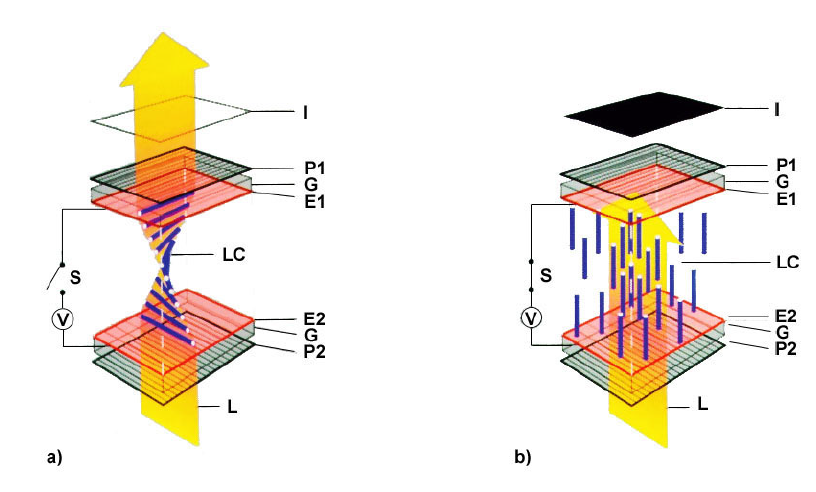
\includegraphics[width=1\linewidth]{images/displayHelix}
			\caption{
			Polarisationsrichtung in der Flüssigkristallanzeige. a) ohne angelegte Spannung. b) bei angelegter Spannung. E1, E2: Elektroden (ITO); G: Glasplatten; I: Lichtintensität; L: Lichtwelle; LC: Flüssigkristall;
P1, P2: Polarisatoren; S: Schalter, V: Spannungsquelle. \cite{displayHelix}
			}
			\label{fig_displayHelixBild}
	\end{figure}

	Dies erlaubt den Bau einer Flüssigkristallanzeige, da in einem Flüssigkristall in cholesterischer Mesophase die Polarisation des Lichtes, wenn es entlang besagter Laufrichtung einfällt, der Helixform des Direktors folgt.
	Wenn bekannt ist, mit welcher Ganghöhe (Länge der Helix bei einer Umdrehung des Direktors) der Kristall vorliegt, kann auf der Ausgangsseite des Displays linear polarisiertes Licht, mit einen Polfilter passieren, wenn dieser zur Einfallsrichtung soweit gedreht ist, wie sich der Direktor über die Dicke des Flüssigkristalls im Display ändert.
	Im Folgenden wird hierfür eine Vierteldrehung verwendet. Wie aus dem Folgenden deutlich wird sind hier nur Drehungen um $\frac{\pi (2z+1)}{2}$ mit $z \in \mathbb{Z}$ praktikabel.
	Da für die lineare Polarisation des einfallenden Lichts ebenfalls ein Polfilter verwendet wird, ist eine solche Flüssigkristallanzeige bidirektional.
	Wenn jetzt im Flüssigkristall ein annähernd homogenes elektrisches Feld angelegt wird, richten sich die Molekülachsen statt nach der Helixstruktur mit zunehmender Feldstärke zunehmend eher nach dem Feld aus.
	Dies verhindert, dass sich die Polarisation des Lichtes im Innern ändert, weshalb bei einer der oben genannten Drehungen der Polarisationsfilter zueinander das Licht den zweiten Polarisationsfilter nicht passieren kann.
	Demnach ist eine spannungsgesteuerte Schaltung der Durchlässigkeit des Filters möglich.

	Flüssigkristalldisplays werden mit Wechselspannung betrieben, da eine Gleichspannung die elektrolytische Zersetzung des Flüssigkristalls zufolge hätte.

	Bei Farbdisplays werden Pixel aus drei Subpixeln zusammengesetzt, welche wiederum aus einer spannungsgesteuerten Flüssigkristallanzeige mit einem Farbfilter (Rot, Grün, Blau) bestehen.

	\par
	Für die Messung wird eine Photodiode verwendet.
	Diese wird über einen Widerstand kurzgeschlossen und die Spannung über den Widerstand gemessen.
	Diese ist im Messbereich proportional zum Photostrom, welcher als im Messbereich proportional zur Intensität des eintreffenden Lichts angenommen wird.
	\par

	\begin{figure}[H]
			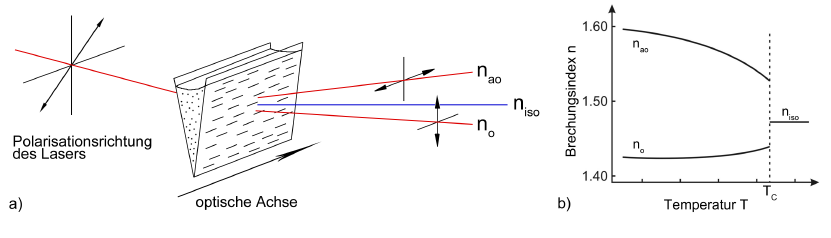
\includegraphics[width=1\linewidth]{images/keil}
			\caption{Schematischer Versuchsaufbau zur Messung der kritischen Temperatur des Übergangs eines Flüssigkristalls von der nematischen in die isotrope Phase. \cite{imp08}
			}
			\label{fig_keil}
	\end{figure}

	Flüssigkristalle weisen einen polarisationsabhängigen Brechungsindex auf, da die Molekülelektronen je nach Orientierung der Moleküle und Schwingungsrichtung sich gegenseitig unterschiedlich stark zum Schwingen anregen. %TODO approven, dunno
	Dies führt bei einem zum Direktor nicht exakt parallelen Strahl zum Phänomen der Doppelbrechung. %TODO approven, dunno
	Der Strahl spaltet in zwei senkrecht zueinander polarisierte Strahlen auf.
	Diese Aufspaltung wird maximal, wenn der einfallende Strahl senkrecht zum Direktor steht.
	Wenn der Flüssigkristall in einem keilförmigen Gefäß ist, behält der Strahl nach dem Austritt aus dem Kristall eine Winkelaufspaltung, weshalb in größerem Abstand die Aufspaltung einfacher gemessen werden kann (vgl. \cref{fig_keil}).
	In einem plan-parallelen Aufbau würden die Strahlen nach dem Austritt aus dem Kristall wieder parallel verlaufen und die Ortsaufspaltung würde nicht mit dem Messabstand steigen.
  Die Differenz der Brechungsindizes ist dabei direkt abhängig vom Ordnungsgrad, weshalb sie als ein Maß für diesen verwendet werden kann.

	Bei steigender Temperatur steigt die mittlere Abweichung der Molekülachsen vom Direktor und damit sinkt der Ordnungsgrad und die Differenz der Brechungsindizes.
	Ab einer bestimmten, materialabhängigen kritischen Temperatur verliert der Flüssigkristall seine Orientierungsfernordnung vollständig und das Phänomen der Doppelbrechung verschwindet.

	\section{Methoden}
	% Bilder von der Website klauen
	% einer will Präsens
	% Doppelbrechung
	% Fernordnungskram und Phasen und bla
	\subsection{Herstellung der Flüssigkristallanzeige}
	Es werden rechteckige Glasplatten verwendet, auf die zuvor eine Schicht aus Indiumzinnoxid aufgebracht wurde.
	Dies erlaubt eine einseitige elektrische Leitfähigkeit der Schichten, die nötig ist, um später ein elektrisches Feld anlegen zu können.
	Die Glasplatten werden zunächst in einem Ultraschallbad von Verunreinigungen auf der Oberfläche befreit.
	Mit einem Multimeter wird die leitende Seite der Platten bestimmt.
	Auf diese Seite werden bei beiden Platten Rillen entlang der langen Seite der Platten durch wiederholtes Reiben mit einem Tuch aufgebracht.
	Dann werden die Platten im \SI{90}{\degree}-Winkel aufeinander gelegt, wobei \SI{15}{\micro \meter} dicke Streifen auf zwei gegenüberliegenden Seiten als Abstandshalter verwendet werden (vgl. \cref{fig_ohnestern}).
	Beim Aufeinanderlegen wird je eine der Ecken der Platten aneinander ausgerichtet, sodass von beiden Platten ein Stück übersteht, an das später der Kontakt angebracht werden kann.
	Der \SI{90}{\degree}-Winkel ist wichtig, damit sich die Flüssigkristallmoleküle daran ausrichten und sich die Helixstruktur der cholesterischen Phase mit der Ganghöhe $p=4h$, wenn $h$ der Abstand der Glasplatten (\SI{15}{\micro \meter}) ist, die Moleküle sich also zwischen den Platten um \SI{90}{\degree} drehen.
	Dann werden zunächst die beiden Seiten mit Abstandshalter mit Zweikomponentenkleber bestrichen, um sie abzudichten und gewartet, bis er ausgehärtet ist.
	Dann wird mit einer Spitze ein Tropfen Flüssigkristall auf eine der noch offenen Seiten gebracht. Für die Verteilung im Innern der Anzeige wird die Kapillarität ausgenutzt.
  Sobald der Flüssigkristall im Innern verteilt ist, werden die übrigen Seiten mit Kleber verschlossen.
	Zuletzt werden Polarisationsfilter im \SI{90}{\degree}-Winkel zueinander auf die Außenseiten der Flüssigkristallanzeige geklebt.

	\begin{figure}[H]
			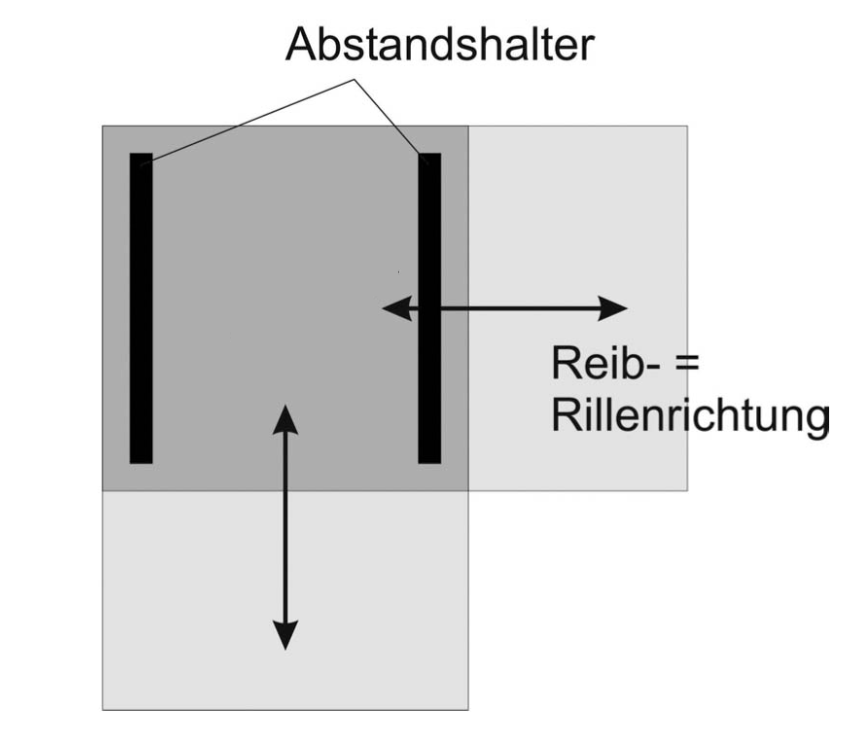
\includegraphics[width=0.5\linewidth]{images/ohnestern.PNG}
			\caption{
			Konstruktionsskizze des LC-Displays \cite{imp08}. Die Rillen in beiden Platten sind um \SI{90}{\degree} gegeneineander verdreht.
			}
			\label{fig_ohnestern}
	\end{figure}

	\subsection{Bestimmung der elektrooptischen Kennline}
	An den überstehenden Flächen der Flüssigkristallanzeige wird über Krokodilklemmen eine Spannung angelegt und zunächst eine qualitative Beobachtung des Verdunklungsvorgangs beim Erhöhen der Spannung von \SIrange{0}{8}{V} durchgeführt.
	Gleiches wird für eine kommerziell erhältliche, industriell gefertigte LC-Anzeige durchgeführt.
	Dann werden die Anzeigen nacheinander zwischen eine Lampe und eine Photodiode gebracht und die Spannung an der Photodiode bei schrittweiser Erhöhung der Spannung an der Anzeige gemessen.

	\subsection{Bestimmung der kritischen Temperatur eines Flüssigkristalls}
	Der Effekt der Doppelbrechung wird ausgenutzt, um die Temperatur zu bestimmen, ab der ein untersuchter Flüssigkristall seine Eigenschaften als solcher (also seine Orientierungsfernordnung) verliert.
	Um die Orientierungsfernordnung indirekt zu messen, wird die Doppelbrechung des Kristalls beobachtet.
	Hierzu wird ein Laserstrahl auf ein keilförmiges Gefäß mit einem Flüssigkristall im Innern gerichtet.
	Durch die Doppelbrechung spaltet dieser in zwei unterschiedlich polarisierte Strahlen auf.
	Jetzt wird mit einem Peltierelement die Temperatur des Flüssigkristalls langsam erhöht und dabei der Abstand der Teilstrahlen mit einem Millimeterpapier gemessen.
	Die Temperatur, ab der der Abstand der Teilstrahlen verschwindet, entspricht der kritischen Temperatur des Phasenübergangs von nematischer zu isotroper Phase.

	\section{Ergebnisse und Diskussion}
	\subsection{Bestimmung der Kennlinien der LC-Displays}
	\subsubsection{Unsicherheiten}
	Beide Spannungen werden von einer digitalen Anzeige abgelesen.
	Mit einer Rechteckverteilung ergibt sich für die Spannung $U_{LCD}$ mit welcher das Display betrieben wird $u(U_{LCD})=\SI{0.00003}{V}$ und für die der Photodiode $u(U_{Ph})=\SI{0.0003}{V}$.
	Da beide Anzeigen stark in den letzten Ziffern schwanken, wird die Breite der Schwankungen mit
	\begin{itemize}
		\item $u(U_{LCD})=\SI{0.001}{V}$
		\item $u(U_{Ph})=\SI{0.003}{V}$
	\end{itemize}
	abgeschätzt, wohingegen die Displayunsicherheiten verschwinden.
	Da die Schwankungen der Diodenspannung deutlich größer im Bereich von 10\% bis 90\% Transmission ist, wird dort die doppelte Unsicherheit verwendet.
	\subsubsection{Beobachtung und Datenanalyse}
	Beim Betrieb des selbst gebauten und industriellen Displays lässt sich feststellen, dass sie dunkler, bzw. weniger lichtdurchlässig, werden, wenn man die angelegte Spannung erhöht.
	Das selbst gebaute Display flimmert und wird auch bei höheren Spannungen nicht so dunkel wie das industriell gefertigte Display.

	Um von der an der Photodiode gemessenen Spannung auf auf die relative Transmission zu schließen wird
	\begin{equation}
			T = \frac{U-U_{max}}{U_{max}-U_{min}}
	\end{equation}
	verwendet, da sie hierdurch auf $0\leq T \leq 1$ normiert wird. Dabei ergibt sich die kombinierte Standardunsicherheit
	\begin{align*}
		u(T) &= \sqrt{\sum_{i}\left(\frac{\partial T}{\partial x_i} u(x_i)\right)^2}\\
		&= \sqrt{\left(\frac{u(U)}{U_{max}-U_{min}}\right)^2+\left(\frac{u(U_{max})(U_{min}-U)}{(U_{max}-U_{min})^2}\right)^2+\left(\frac{u(U_{min})(U-U_{max})}{(U_{max}-U_{min})^2}\right)^2} \\
		&=	\frac{\sqrt{ (\alpha^2+1) (U_{max}-U_{min})^2+2U_{max}U_{min}+2U(U-U_{max}-U_{min})}}{(U_{max}-U_{min})^2} u(U_{max}), \\
	\end{align*}
	wobei
	\begin{equation*}
			u(U)=\alpha u(U_{max})=\alpha u(U_{min})
	\end{equation*}
	verwendet wurde.

	Mittels der Werte aus \cref{tb_maxmin} lassen sich die Messpunkte in die Kennlinien in \cref{fig_industry} und \cref{fig_selfmade} transformieren.
\begin{table}[H]
		\centering
		\begin{tabular}{ c | c | c }
			 & industriell & selbst gebaut \\ \hline
			$U_{max}$ & \SI{2.414+-0.003}{V} & \SI{1.866+-0.003}{V} \\
			$U_{min}$ & \SI{0.047+-0.003}{V} & \SI{0.360+-0.003}{V} \\
	%\hline
		\end{tabular}
		\caption{Maximal und minimal gemessene Spannungen beim Bestimmen der Kennlinie des selbst gebauten und industriell gefertigten Displays mittels einer Photodiode.}
		\label{tb_maxmin}
\end{table}

	\begin{figure}[H]
			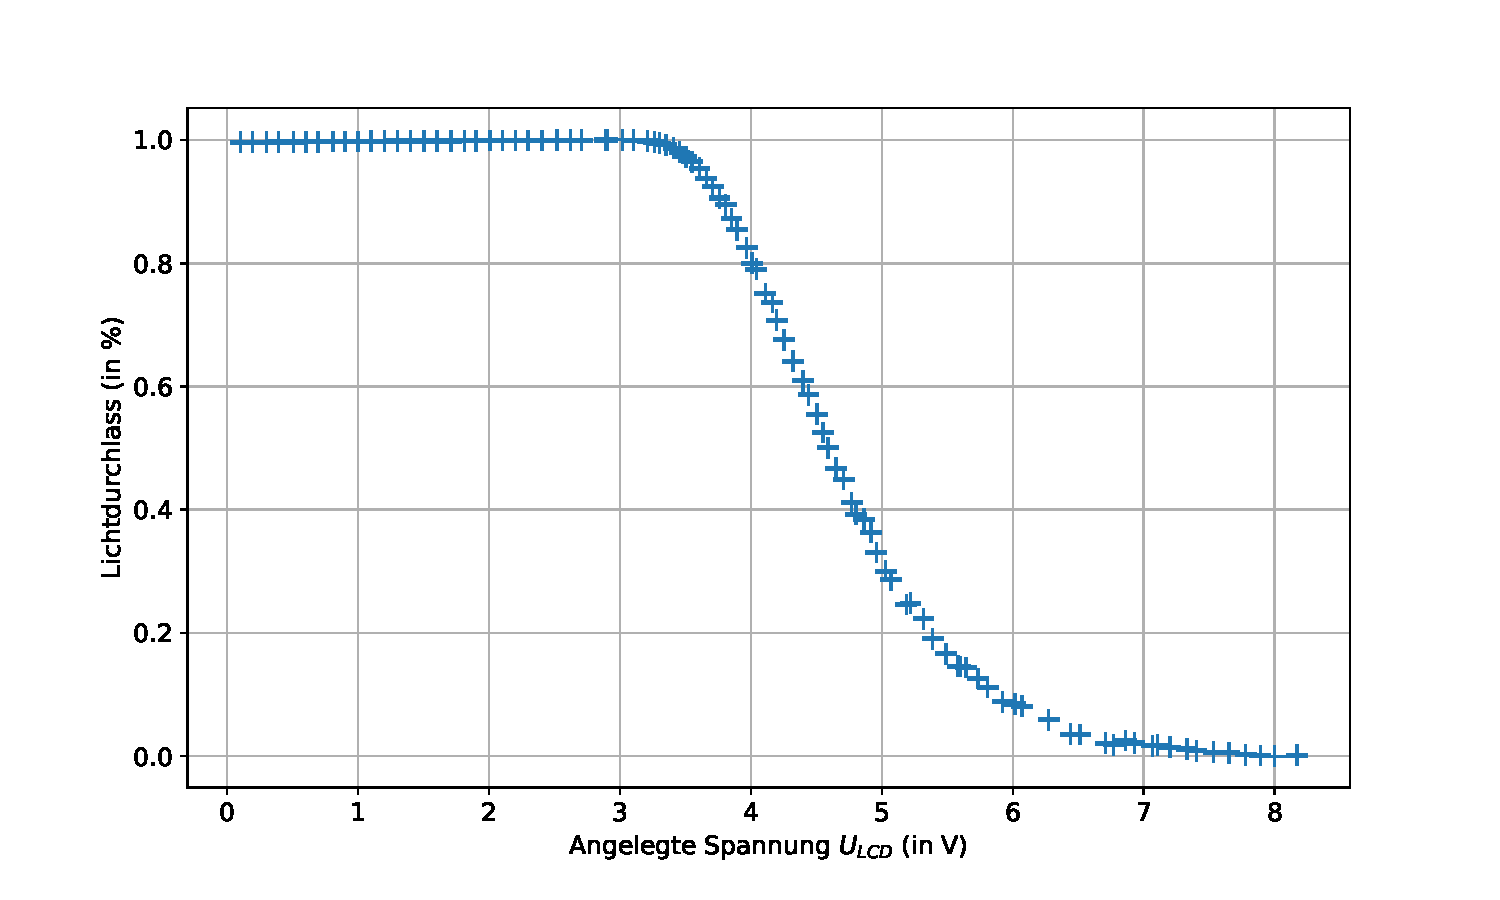
\includegraphics[width=1\linewidth]{images/industry.pdf}
			\caption{Kennlinie des industriell hergestellten LC-Displays.
			Die schwarze Senkrechte liegt bei der Schwellspannung, welche mindestens am Display anliegen muss, um einen Unterschied in der Transmissivität messen zu können.
			Die rote(grüne) dagegen liegt bei der Spannung, bei der eine Transmission von 90\%(10\%) durch das Diplay gemessen wurde.
			}
			\label{fig_industry}
	\end{figure}
	\begin{figure}[H]
			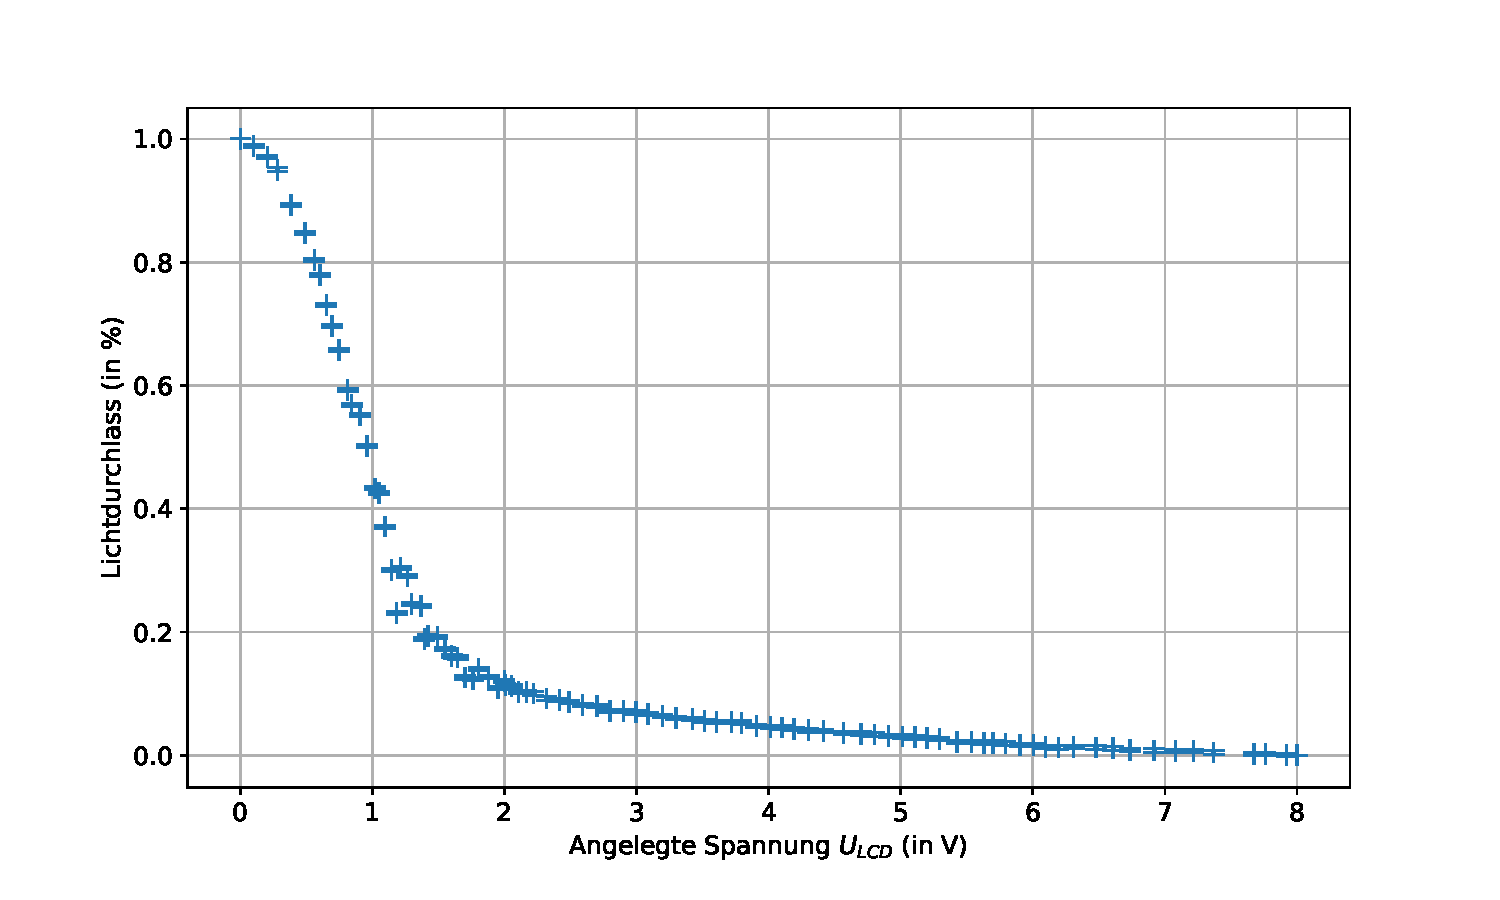
\includegraphics[width=1\linewidth]{images/selfmade.pdf}
			\caption{Kennlinie des selbst gebauten LC-Displays.
			Die schwarze Senkrechte liegt bei der Schwellspannung, welche mindestens am Display anliegen muss, um einen Unterschied in der Transmisivität messen zu können.
			Die rote(grüne) dagegen liegt bei der Spannung, bei der eine Transmission von 90\%(10\%) durch das Diplay gemessen wurde.
			}
			\label{fig_selfmade}
	\end{figure}
	Aus den Kennlinien lassen sich die Kenngrößen aus \cref{tb_kenngroessen} bestimmen.
	\begin{table}[H]
		\centering
		\begin{tabular}{ c | c | c }
			 & industriell & selbst gebaut \\ \hline
			$\Delta U=U_{10}-U_{90}$&\SI{2.0009+-0.0016}{V}&\SI{1.8348+-0.0016}{V} \\
			$U_{th}$ & \SI{3.211+-0.0012}{V} & \SI{0.0016+-0.0012}{V} \\
			\hline
		\end{tabular}
		\caption{Kenngrößen des selbst gebauten und industriell gefertigten Displays.}
		\label{tb_kenngroessen}
\end{table}

	\subsubsection{Diskussion}
	Zunächst einmal muss angemerkt werden, dass der hier bestimmte Wert für $\Delta U=U_{10}-U_{90}$ zwar erlaubt zu klassifizieren, ob das Display besser dazu geeignet ist, technisch einfach viele Helligkeitsstufen darzustellen oder aber mit geringer Spannungsdifferenz eine kontrastreiche Hell-Dunkel-Anzeige zu realisieren.
	Ob das Display tatsächlich gut für eine der beiden Varianten geeignet ist, hängt aber auch davon ab, wie hoch die Differenz der nichtnormierten Transmissivität bei $U_{max}$ und $U_{max}$ ist, da dies den tatsächlichen Kontrast beschreibt, also wie gut das durchsichtig geschaltete Display von undurchsichtigen zu unterscheiden ist.

	Wenn man zunächst nur die erste Überlegung anwendet, stellt man fest, dass das industrielle Display eine größere Spannungsdifferenz (\SI{2.0009+-0.0016}{V}) zum Schalten benötigt, also besser für ein Display mit vielen verschiedenen Helligkeitsstufen geeignet ist, als das selbst gebaute, während dieses nur eine geringe Spannungsdifferenz (\SI{1.8348+-0.0016}{V}) benötigt und somit z.B. für Taschenrechner, deren Batterien eine geringe Spannung liefern, geeignet ist.
	Letztere Einschätzung verstärkt sich dadurch, dass das industrielle bereits eine deutlich höhere Schwellspannung (vgl. \cref{tb_kenngroessen}) benötigt, um überhaupt in den schaltbaren Bereich zu kommen.
	Wenn man allerdings die nichtnormierte Spannung an der Diode als Rückschluss auf die Intensität und diese als Rückschluss auf die nichtnormierte Transmissivität betrachtet (vgl. \cref{tb_maxmin}), stellt man fest, dass die industrielle Anzeige, wenn sie auf lichtdurchlässig geschaltet ist, deutlich mehr Licht durchlässt und im undurchlässigen Fall deutlich weniger passieren lässt als die selbst gebaute.
	Dies bedeutet, dass, wenn man die nötige Spannung aufbringen kann, auch für eine Hell-Dunkel-Anzeige die industrielle Anzeige für ein einfaches Ablesen deutlich besser geeignet ist.
	Die geringe Schwellspannung hat zusätzlich den Nachteil, dass  Spannungsschwankungen im durchlässigen Modus die Helligkeit des Displays ändern.
	%TODO FLackern, aber kp

	Die geringere Transmissivität der selbst gebauten im durchlässigen Fall kann darin begründet sein, dass die selbst gebaute Anzeige stärker verunreinigt ist, ein anderer Flüssigkristall verwendet wurde oder das elektrische Feld im Innern des Displays aufgrund von Widerstandsverlusten geringer ist.
	Die höhere Transmissivität der selbst gebauten im undurchlässigen Fall kann auf ein höhere Schichtdicke des Flüssigkristalls oder eine bessere Ausrichtung der Moleküle an den Glasplatten im industriellen Display zurückgeführt werden.
	Außerdem ist zu erwarten, dass die Polfilterfolie nicht exakt im \SI{0}{\degree}-Winkel zu den Rillen in der Glasplatte aufgeklebt wurde, welche zueinander wiederum nicht exakt parallel sind.

	Dass es sich um einen anderen Flüssigkristall handelt kann dadurch bestätigt werden, dass sich die Schwellspannungen so stark unterscheiden, da die Schwellspannung mit der dielektrischen Anisotropie sinkt, welche davon abhängt, um welchen Flüssigkristall es sich handelt.
	% habe noch mal gedenkt, könnte der industrielle nicht auch einfach nur nen fake widerstand drin haben zum Trollen? > ja, aber würde ich nicht vermutetn

	\subsection{Bestimmung der kritischen Temperatur eines Flüssigkristalls}
	\subsubsection{Unsicherheiten}
	Die Temperatur des Flüssigkristalls wird mit einem Thermometer mit einer Nachkommastelle gemessen, wodurch sich eine Unsicherheit von $u(T)=\SI{0.03}{\celsius}$ ergibt.
	Die Unsicherheit des Abstands der aufgespalteten Strahlen des Lasers wird mit $u(d)=\SI{1.7}{mm}$ abgeschätzt.
	Diese setzt sich aus dem Durchmesser des Laserstrahlquerschnitts auf dem Millimeterpapier und der instabilen Halterung des Laserpointers zusammen.
	\subsubsection{Beobachtung und Datenanalyse}
	Beim Steigern der Temperatur des Flüssigkristalls zeigt sich zunächst kaum eine Änderung in der Aufspaltung des Laserstrahls.
	Erst beim Überschreiten einer Grenztemperatur ändert sich die milchige Farbe des Kristalls zu der einer klaren Flüssigkeit.
	Zeitgleich verschwinden die zwei Strahlen und es findet sich nur noch ein Strahl zwischen den Positionen der ursprünglichen Strahlen.

	Der gemessene Abstand der Laserstrahlen ist in \cref{fig_laser} abhängig von der Temperatur dargestellt.
	Die kritische Temperatur $T_C$ liegt demnach bei \SI{36.0+-0.6}{\celsius }.
	\begin{figure}[H]
			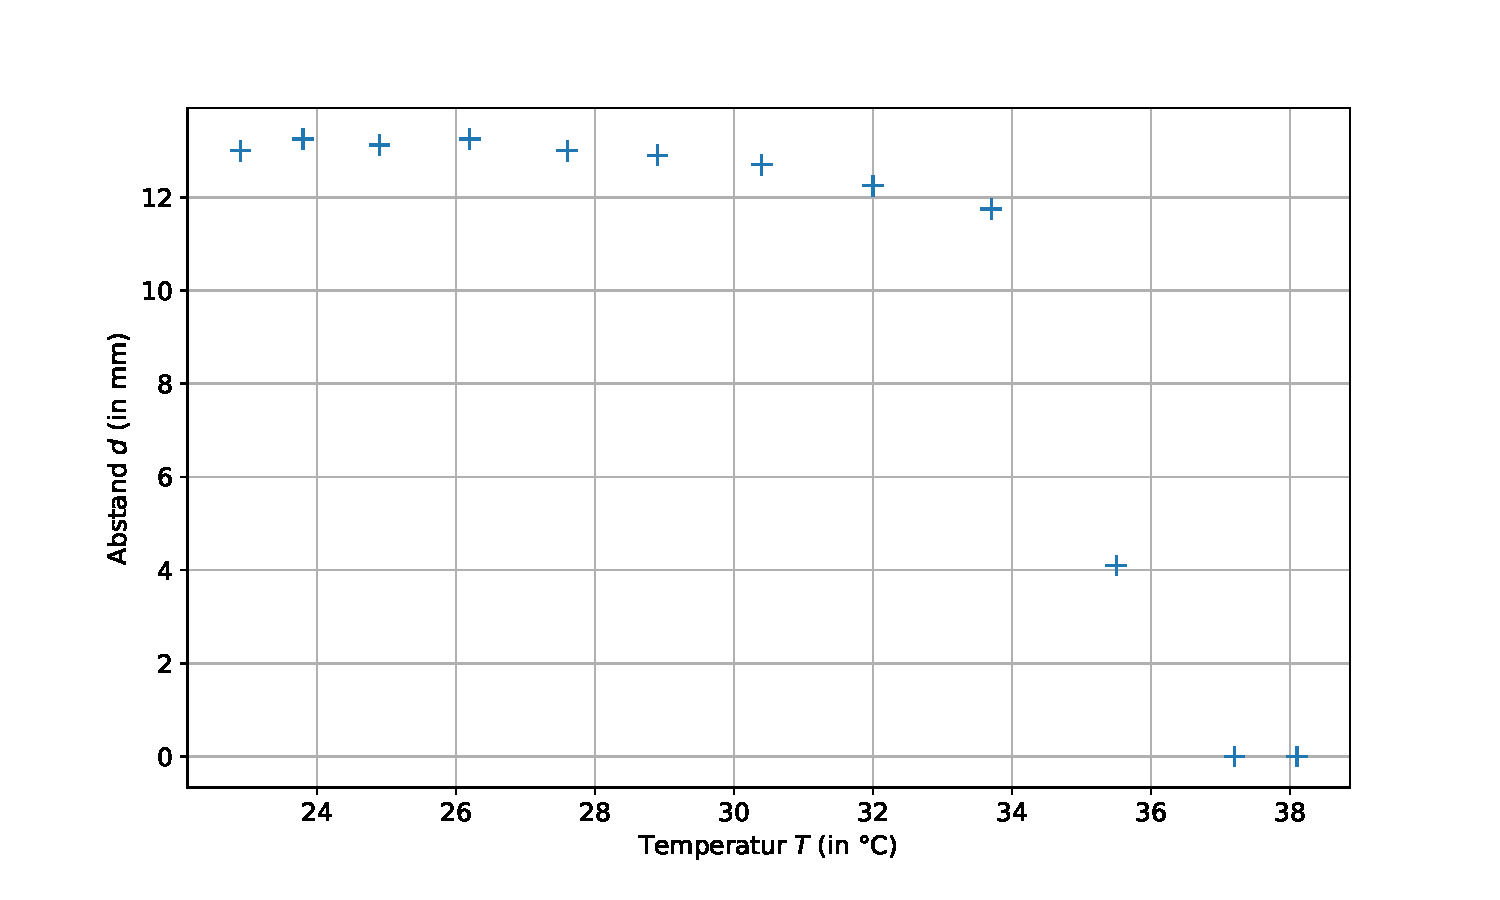
\includegraphics[width=1\linewidth]{images/laser.pdf}
			\caption{
			Temperaturabhängigkeit des Flüssigkristalls.
			}
			\label{fig_laser}
	\end{figure}
	\subsubsection{Diskussion}

	Zu \cref{fig_laser} lässt sich sagen, dass der Sprung von der nematischen Phase in die isotrope deutlich weniger abrupt vonstatten geht, als zu erwarten war.
	Diese Erwartung geht darauf zurück, dass es für den Kristall am energetisch günstigsten ist, erst dann die Orientierungsfernordnung zu verlieren, wenn die kritische Temperatur überschritten ist und davor bei homogener Temperatur zwar steigende, aber geringe Abweichungen von der Orientierungsfernordnung stattfinden. %TODO confirmen pls
	Aufgrund der Art und Weise, wie die Peltierelemente positioniert sind, kann jedoch angenommen werden, dass die Temperatur im Innern des Flüssigkristalls nicht homogen ist und somit Teile des Kristalls bereits die Orientierungsfernordnung verloren haben, während andere sie noch haben.

	Dies erklärt den Messpunkt in \cref{fig_laser} bei etwa $T= \SI{35,5}{\celsius}$, da hier offenbar der Laser durch einen Teil Flüssigkristall mit und einen ohne Orientierungsfernordnung strahlt und somit die Aufspaltung geringer ist, als wenn er vollständig durch Flüssigkristall in nematischer Phase strahlt.

	Dass der Kristall bei der gleichen Temperatur klar wird, bei der die Doppelbrechung verschwindet, entspricht der Erwartung, da die Doppelbrechung für die milchige Farbe verantwortlich ist.

	Aus dieser Feststellung lässt sich folgern, dass diese Methode mit dem verwendeten Aufbau nur geeignet ist, um eine grobe Bestimmung der kritischen Temperatur durchzuführen.
  Die so bestimmte Temperatur beträgt \SI{36.0+-0.6}{\celsius} und beinhaltet im doppelten Unsicherheitsintervall den Literaturwert von 4’-Pentyl[1,1’-biphenyl]-4-carbonitril (5CB) aus \cite{Luk2004} von \SI{35}{\celsius}.

	Ein längeres Warten vor der Aufnahme des Messwertes würde nur bedingt hiergegen helfen, da durch die Positionierung der Peltierelemente immer noch ein räumliches Temperaturgefälle zwischen Peltierelement und Umgebungsluft bestehen würde.
	Dies könnte nur durch ein gleichmäßiges Erhitzen der gesamten Umgebung des Versuchsaufbaus umgangen werden.

	% Allgemeine Beobachtungen
	% Einflüsse von veränderten Parametern auf Messung
	% Berechung nach Aufgabenstellung

	% Bezug/Nutzen oder sonst was
	% auch hier die Hypothese wiederholen
	% keine Messwerte hier, nach manchen Menschen, zumindest "direkt" erstellte Diagramme net hier, auch wenn Lesbarkeit-bla

	\section{Schlussfolgerung}
	% Rückgriff auf Hypothese und drittes Nennen dieser

	Zusammengefasst lässt sich feststellen, dass eine Flüssigkristallanzeige hergestellt werden konnte, ihre elektrooptische Kennlinie aufgenommen werden konnte sowie die kritische Temperatur des Übergangs zwischen nematischer und isotroper Phase eines anderen Flüssigkristalls bestimmt werden konnte.
	Beim Vergleich der selbst gebauten Flüssigkristallanzeige mit einer industriellen wurde festgestellt, dass die selbst gebaute in ihren Eigenschaften für die Anwendung schlechter geeignet ist als die industrielle.
	Lediglich in Bezug auf die Geringe der Schwellspannung ist die selbst gebaute im Vorteil.
	Die Bestimmung der kritischen Temperatur eines Flüssigkristalls durch Ausnutzung der Doppelbrechung war möglich, aber aufgrund der Art der Versuchsdurchführung und des Versuchsaufbaus nur innerhalb großer Unsicherheiten.
	Für eine genauere Untersuchung wäre ein langsameres Erhöhen der Temperatur in geringeren Schritten und die Möglichkeit eines gleichmäßigeren Erhitzens des Flüssigkristalls notwendig.
	% Ein Literaturwertvergleich war hier leider nicht möglich, da nicht bekannt ist, um welchen Flüssigkristall es sich handelt.

	% Quellen zitieren, Websiten mit Zugriffsdatum
	% Verweise auf das Laborbuch (sind erlaubt)
	% Tabelle + Bilder mit Beschriftung
	\printbibliography
\end{document}
%TODO selbst gebaut wird von Duden über selbstgebaut empfohlen
